\chapter{Các kết quả thí nghiệm}
\label{Chapter4}

\textit{Trong chương này, chúng tôi trình bày các kết quả thí nghiệm nhằm đánh giá những nội dung đã trình bày ở Chương 3. Cho các thí nghiệm về nguyên lý, chúng tôi sử dụng dữ liệu được tạo ngẫu nhiên và hàm lỗi Mean Squared Error; với các thí nghiệm thực tế, chúng tôi sử dụng bộ dữ liệu MNIST và CIFAR10 và hàm lỗi Cross Entropy. Kết quả thí nghiệm cho thấy thuật toán mà chúng tôi cài đặt có thể xấp xỉ kết quả mà bài báo công bố, tuy nhiên chúng tôi nhận thấy rằng bộ siêu tham số được sử dụng để tái tạo kết quả có thể không cho kết quả tốt nhất cho tất cả thuật toán. Ngoài ra, các kết quả thí nghiệm cũng cho thấy các trường hợp mà các thuật toán khác gặp khó khăn, và cách mà Adam vượt qua các khó khăn đó. Cuối cùng, các thí nghiệm cho thấy tốc độ tối ưu hóa của các thuật toán trên các mô hình mạng nơ-ron thực tế với nhiều tầng ẩn gồm các cấu trúc khác nhau.}

\section{Các thiết lập thí nghiệm}

Chúng tôi thực hiện hai loại thí nghiệm: thí nghiệm nguyên lý và thí nghiệm thực tế. Trong các thí nghiệm nguyên lý, chúng tôi sử dụng hàm số để tạo ra dạng địa hình bề mặt lỗi mong muốn. Ngoài ra, chúng tôi cũng tạo một bộ dữ liệu ngẫu nhiên cho các thí nghiệm sử dụng minibatch. Với các thí nghiệm thực tế, chúng tôi sử dụng nhiều bộ dữ liệu khác nhau cùng với các kiến trúc mạng nơ-ron nhiều tầng ẩn được sử dụng để giải quyết các bài toán ứng dụng hiện nay. Những bộ dữ liệu thực tế mà chúng tôi sử dụng:

\begin{itemize}
	\item MNIST \cite{lecun2010mnist}: Bộ dữ liệu này gồm các ảnh xám của các chữ số viết tay từ 0 đến 9 có kích thước 28x28. Tập dữ liệu gồm 60000 ảnh huấn luyện và 10000 ảnh kiểm tra.
	\item CIFAR10 \cite{krizhevsky2009cifar10}: Bộ dữ liệu này gồm các ảnh màu của 10 lớp đối tượng có kích thước 32x32. Tập dữ liệu có tổng cộng 60000 ảnh, mỗi lớp đối tượng có 6000 ảnh. Trong đó 50000 ảnh được chọn làm ảnh huấn luyện và 10000 ảnh kiểm tra. Bộ dữ liệu này và MNIST là những bộ dữ liệu cơ bản phổ biến để huấn luyện các thuật toán học máy và mạng nơ-ron nhiều tẩng ẩn đơn giản.
	\item ImageNet \cite{deng2009imagenet}: Đây là một trong những bộ dữ liệu hình ảnh lớn nhất hiện nay, thường được dùng để kiểm tra khả năng của các phương pháp thị giác máy tính mới nhất. Phiên bản của bộ dữ liệu mà chúng tôi sử dụng là phiên bản được sử dụng trong thử thách ImageNet Large Scale Visual Recogition Challenge 2012 (ILSVRC2012), với hơn 1.2 triệu ảnh được gán nhãn vào 1000 lớp đối tượng được sử dụng để huấn luyện, và 50000 ảnh để kiểm thử.
	\item Penn Tree Bank \cite{marcus1993ptb}: Đây là bộ dữ liệu do Marcus và cộng sự tổng hợp gồm 929 000 từ dùng để huấn luyện, 73 000 từ cho tập kiểm thử và 82 000 từ để kiểm tra. Tập dữ liệu gồm có 10 000 từ trong tập từ điển. Tập dữ liệu đã được qua xử lý được lấy từ trang web của Tomas Mikolov (\url{http://www.fit.vutbr.cz/~imikolov/rnnlm/simple-examples.tgz}).
\end{itemize}

Chúng tôi sử dụng ngôn ngữ lập trình Python và thư viện Numpy cho các thí nghiệm nguyên lý, thư viện Pytorch cho các thí nghiệm thực tế. Cả thư viện Numpy và Pytorch đều cung cấp khả năng tăng tốc thực thi bằng việc véc-tơ hóa tính toán trên nền C/C++. Thư viện Numpy tập trung vào các chức năng tính toán đại số trên CPU, phù hợp với các thí nghiệm đơn giản; trong khi thư viện Pytorch là một thư viện máy học có thể xây dựng các mạng nơ-ron nhiều tầng ẩn phức tạp cùng với khả năng thực thi song song trên GPU. Loại GPU mà chúng tôi sử dụng là NVIDIA RTX 2080, ngoài ra chúng tôi cũng sử dụng NVIDIA Tesla T4 và Cloud Tensor Processing Unit trên nền tảng Google Colaboratory.

Trong tất cả các thí nghiệm, tất cả các thuật toán tối ưu đều có chung điểm xuất phát: bộ trọng số ban đầu đầu của mạng nơ-ron nhiều tầng ẩn sau khi khởi tạo ngẫu nhiên lần đầu sẽ được lưu lại; và với mỗi thuật toán tối ưu được thử nghiệm, bộ trọng số này sẽ được nạp lại vào mạng nơ-ron rồi từ đó mới bắt đầu tiến hành tối ưu và ghi nhận lại kết quả. Điều này giúp đảm bảo sự công bằng cho tất cả các thuật toán khi tiến hành thử nghiệm, tránh được trường hợp một thuật toán nào đó "may mắn" được bắt đầu ở một điểm thuận lợi hơn và nhờ vậy mà hội tụ nhanh hơn.

\begin{center}
	\begin{table}
		\begin{tabular}{|l|c|c|c|}
			\hline
			Thuật toán & Tỉ lệ học & Momentum / $Beta_1$ & Alpha / $Beta_2$ \\
			\hline
			SGD & [0.0001, 0.1] & - & - \\
			\hline
			Momentum & [0.0001, 0.1] & [0.1, 0.99] & - \\
			\hline
			Adagrad & [0.0001, 0.1] & - & - \\
			\hline
			RMSprop & [0.0001, 0.1] & - & [0.9, 0.999] \\
			\hline
			Adam & [0.0001, 0.1] & [0.1, 0.99] & [0.9, 0.999] \\
			\hline
		\end{tabular}
	\caption{\label{tab:hparam-search}Khoảng giá trị để dò tìm siêu tham số tốt nhất của các thuật toán tối ưu.}
	\end{table}
\end{center}

\section{Các kết quả thí nghiệm}

\subsection{Kết quả của thuật toán cài đặt so với bài báo}

Trong phần này, chúng tôi trình bày kết quả của các thuật toán tối ưu mà chúng tôi cài đặt. Cụ thể, chúng tôi so sánh kết quả của các thuật toán do chúng tôi cài đặt lại trên nền thư viện Pytorch với kết quả được công bố trong bài báo trong thí nghiệm Multi-layer Neural Network trên tập dữ liệu MNIST và thí nghiệm Convolutional Neural Network trên tập dữ liệu CIFAR10. Việc tái tạo các kết quả được công bố gặp nhiều khó khăn do bản chất ngẫu nhiên của SGD và dropout, cộng với việc tác giả không công bố các siêu tham số cho các thí nghiệm cũng như các cài đặt liên quan khác. Bài báo cũng không đề cập các khoảng tìm kiếm cho quá trình tìm siêu tham số tối ưu nhất của mỗi thuật toán, vì vậy chúng tôi đã tham khảo các công trình nghiên cứu khác sử dụng các tối ưu này, và tổng hợp các giá trị nhỏ nhất và lớn nhất cho từng siêu tham số của mỗi thuật toán để làm khoảng tìm kiếm (bảng \ref{tab:hparam-search}). Bài báo thực hiện thí nghiệm với thuật toán Nesterov \cite{nesterov1983amf}, Adagrad, RMSprop, AdaDelta \cite{zeiler2012adadelta} và Adam; tuy nhiên chúng tôi nhận thấy rằng Nesterov và AdaDelta không liên quan trực tiếp đến thuật toán Adam mà khóa luận tập trung tìm hiểu, vì vậy chúng tôi sẽ tập trung thực hiện thí nghiệm trên các thuật toán SGD, Momentum, Adagrad, RMSprop, và Adam.

Trong thí nghiệm ``Multi-layer Neural Network'', kết quả mà chúng tôi cài đặt so với kết quả được công bố trong bài báo xấp xỉ nhau về đường đi và vị trí tương đối giữa các thuật toán với nhau (hình \ref{fig:exp-mlp}). Tuy nhiên, giá trị loss trong cài đặt của chúng tôi cũng thấp hơn đáng kể so với kết quả trong bài báo.

\begin{figure}[htp]
	\centering
	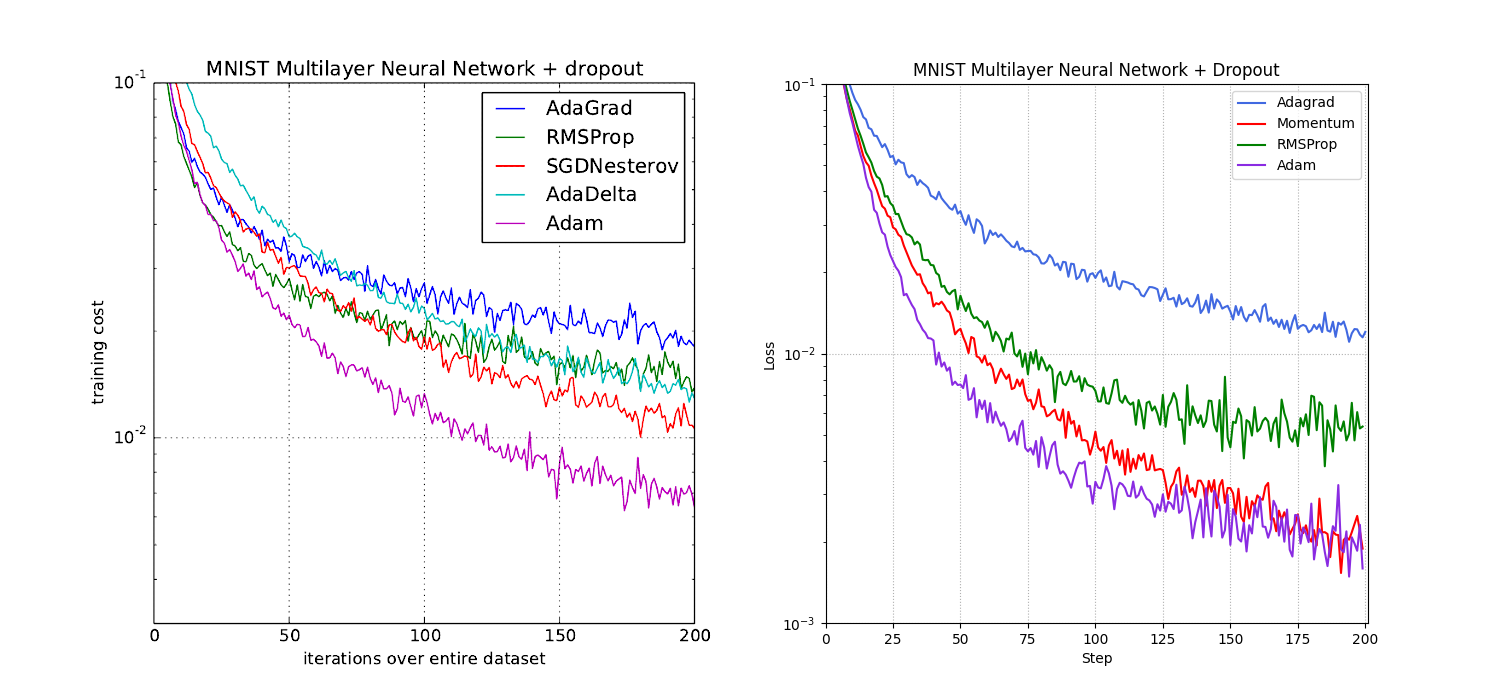
\includegraphics[width=140 mm]{images/mlp.png}
	\caption{Kết quả thí nghiệm Multi-layer Neural Network giữa thuật toán mà chúng tôi cài đặt so với bài báo. Bên trái: kết quả mà bài báo công bố. Bên phải: kết quả do chúng tôi tự cài đặt lại.}
	\label{fig:exp-mlp}
\end{figure}

Nhìn chung, thuật toán Adam có tốc độ tối ưu độ lỗi nhanh nhất trong tất cả các thuật toán được thử nghiệm. Điểm yếu của Adagrad về tỉ lệ học luôn giảm dần được thể hiện rõ khi Adagrad chuyển hướng đi ngang dần mặc dù độ lỗi vẫn cao trong khi các thuật toán khác tiếp tục đi xuống. Điều đó cho thấy rằng mô hình vẫn đang trong quá trình học dữ liệu, nhưng vì tỉ lệ học quá nhỏ nên ở mỗi bước, lượng cập nhật trọng số không đủ để cải thiện mô hình. Vấn đề tỉ lệ học giảm dần do cộng dồn gradient bình phương của Adagrad được RMSprop khắc phục bằng một tỉ lệ suy biến, giúp RMSprop bắt kịp gần hơn với Momentum và Adam. Thuật toán Momentum là thuật toán có kết quả khác biệt nhất giữa cài đặt của chúng tôi và cài đặt trong bài báo. Nếu như trong bài báo, Momentum khá xấp xỉ với RMSprop thì chúng tôi lại ghi nhận được rằng Momentum luôn luôn có độ lỗi tốt hơn RMSprop, và thậm chí còn bắt kịp với Adam ở những bước cuối cùng.

Trong thí nghiệm ``Convolutional Neural Network'', chúng tôi cũng thực hiện tìm bộ siêu tham số đem lại kết quả cuối cùng thấp nhất cho mỗi thuật toán. Tuy nhiên, sau khi đã tìm được những bộ siêu tham số cho tất cả các thuật toán và thực hiện thí nghiệm, chúng tôi thấy được rằng hầu hết các thuật toán trong cài đặt của chúng tôi đều giúp mô hình đạt được độ lỗi thấp hơn đáng kể so với bài báo khi không dùng dropout. Các giá trị siêu tham số được sử dụng được trình bày chi tiết trong bảng \ref{tab:cnn-hparam}.

Từ hình \ref{fig:exp-cnn-best}, chúng ta có thể thấy rằng bề mặt lỗi của thí nghiệm này có một đoạn dốc xuống khá rõ rệt, và các thuật toán SGD, Momentum cũng như Adam đều giảm độ lỗi rất nhanh khi tìm thấy đoạn dốc ấy. Trong bài báo gốc, một số thuật toán tìm thấy đoạn dốc này ngay từ những epoch đầu tiên, trong khi cài đặt của chúng tôi chỉ bắt đầu giảm mạnh từ khoảng epoch thứ 15. Trong kết quả của chúng tôi, SGD là thuật toán đầu tiên tìm ra đoạn dốc, nhưng độ lỗi tại epoch cuối lại hơi cao hơn so với Momentum và Adam, có thể là do SGD bị giới hạn bởi tỉ lệ học trong khi hai thuật toán kia có cơ chế tăng tốc và đạt được độ lỗi thấp.

\begin{figure}[H]
	\centering
	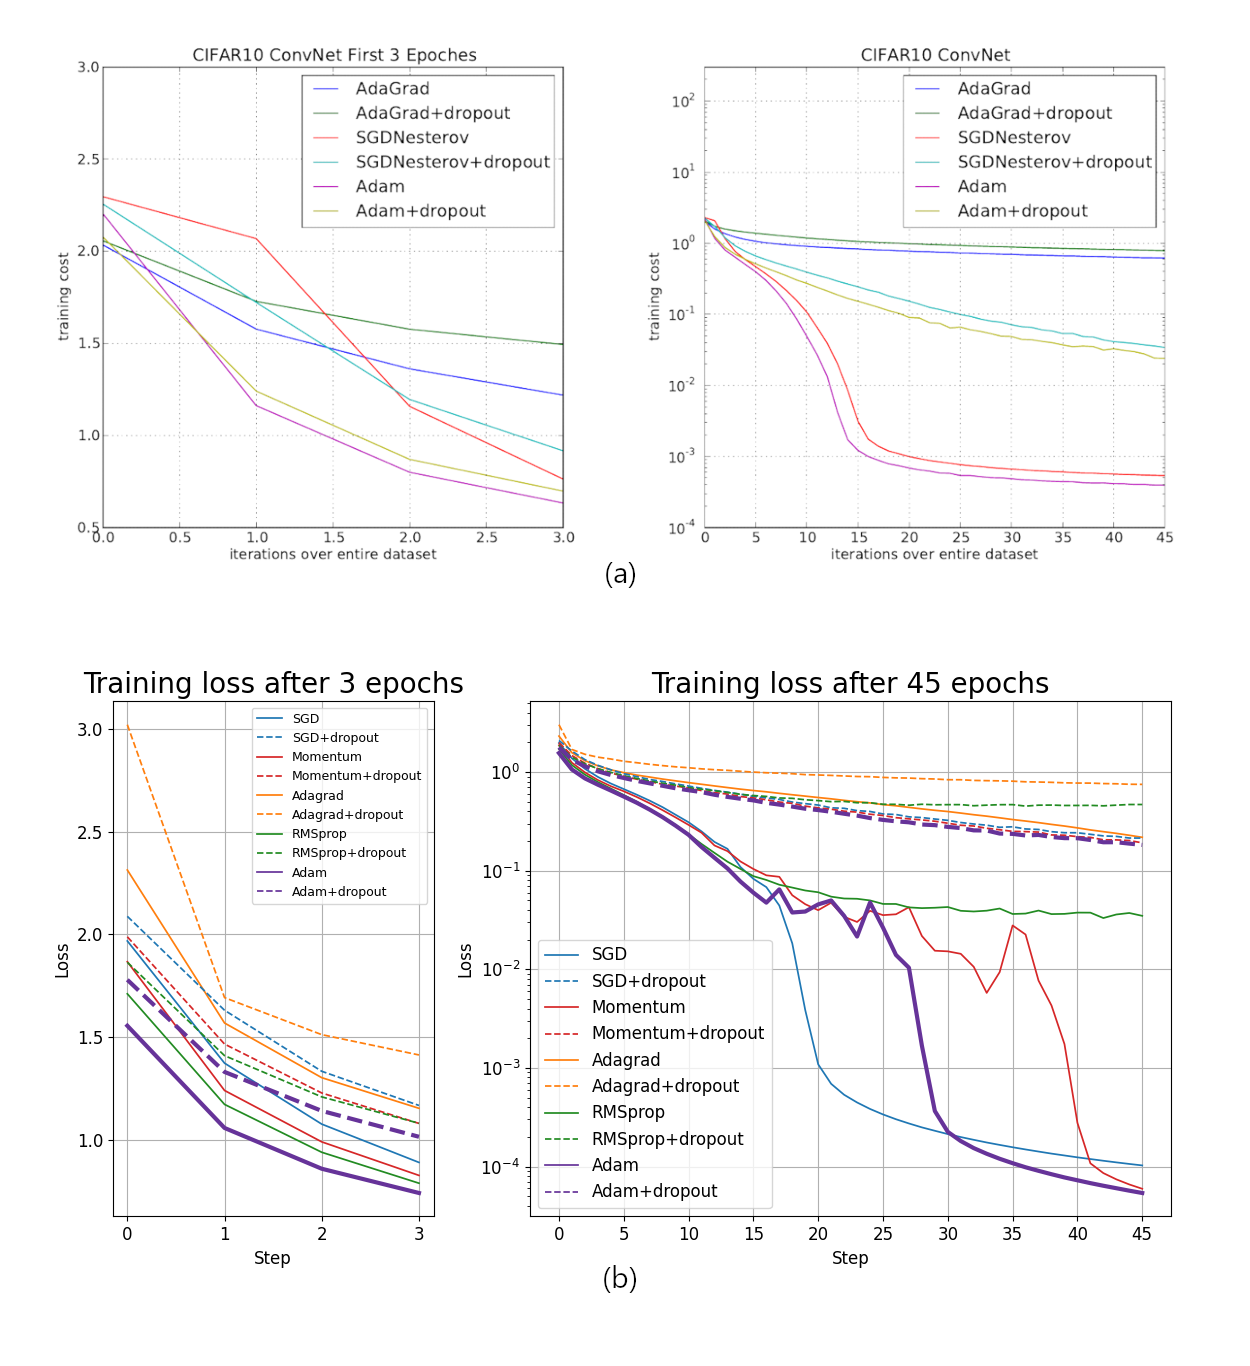
\includegraphics[width=140 mm]{images/cnn.png}
	\caption{Kết quả thí nghiệm Convolutional Neural Network giữa thuật toán mà chúng tôi cài đặt so với bài báo. (a): kết quả mà bài báo công bố. (b): kết quả do chúng tôi tự cài đặt lại.}
	\label{fig:exp-cnn-best}
\end{figure}

Ngoài việc tìm bộ siêu tham số cho kết quả tốt nhất, chúng tôi cũng cố gắng tái tạo kết quả mà bài báo đã công bố. Chúng tôi thực hiện quá trình tái tạo này để kiểm tra tính khả thi của các kết quả mà bài báo đã công bố. Hình \ref{fig:exp-cnn-rep} là kết quả sát nhất với bài báo mà chúng tôi có thể tái tạo được từ khoảng tìm kiếm mà chúng tôi sử dụng. Có thể thấy được rằng, đường đi của các thuật toán trong hình \ref{fig:exp-cnn-best}a và \ref{fig:exp-cnn-rep} có dạng khá giống nhau. Mặc dù có thể tái tạo được hình dạng biểu đồ của các thuật toán, độ lỗi cuối cùng của các thuật toán trong hình \ref{fig:exp-cnn-rep} vẫn cao hơn so với kết quả tốt nhất mà chúng tôi ghi nhận được ở hình \ref{fig:exp-cnn-best}b. Kết quả độ lỗi và thời gian thực thi được trình bày trong bảng \ref{tab:cnn-results}.

\begin{figure}[htp]
	\centering
	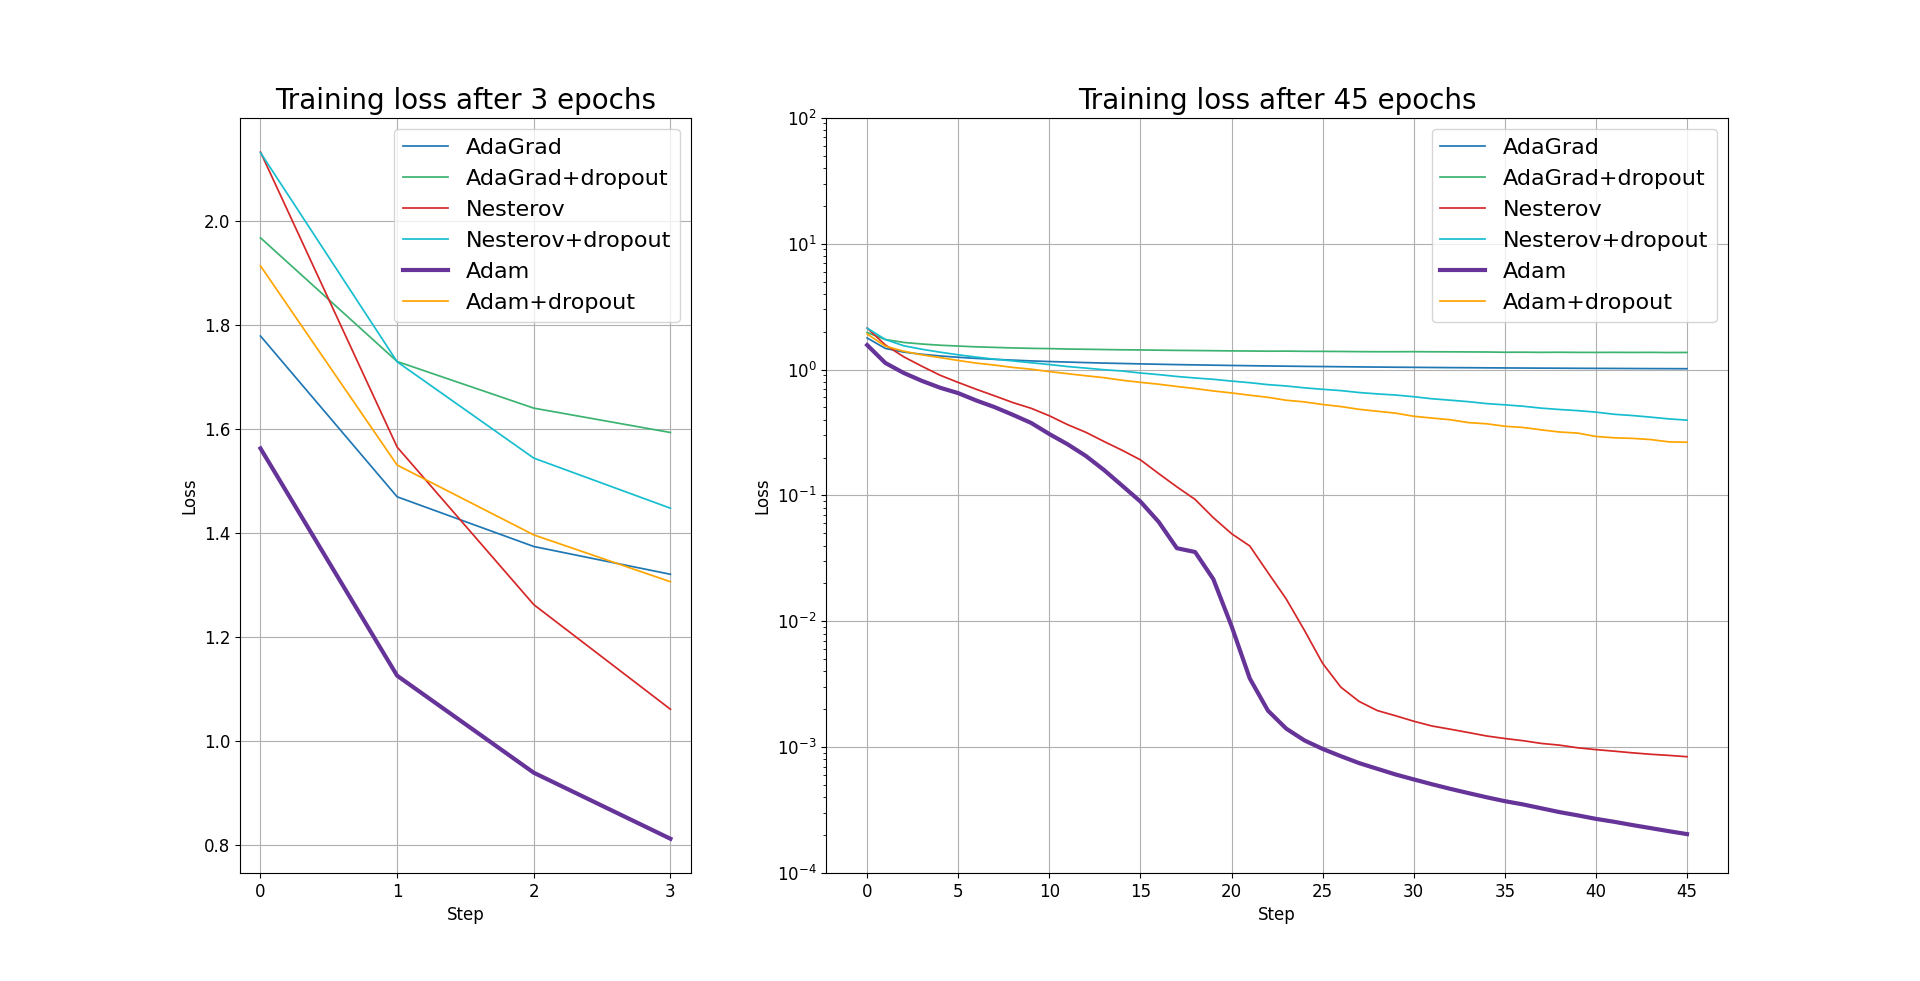
\includegraphics[width=140 mm]{images/cnn-rep.png}
	\caption{Kết quả thí nghiệm Convolutional Neural Network giữa thuật toán mà chúng tôi cài đặt với bộ siêu tham số mô phỏng kết quả của bài báo.}
	\label{fig:exp-cnn-rep}
\end{figure}

Ngoài lí do tác giả không công bố siêu tham số, cũng như tính chất ngẫu nhiên của SGD, một nguyên nhân khả thi khác cho sự khác biệt giữa kết quả mà chúng tôi ghi nhận được so với kết quả mà bài báo công bố là bản chất cài đặt của thư viện. Mỗi thư viện có cách xử lý tính toán riêng dẫn đến kết quả có phần lệch nhau. Vì tác giả cũng không nói rõ thư viện được sử dụng trong bài báo, nên thư viện Pytorch mà chúng tôi sử dụng có thể sẽ ra kết quả khác so với bài báo.

\begin{table}
	\begin{tabular}{|l|m{0.18\textwidth}|m{0.18\textwidth}|m{0.18\textwidth}|}
		\hline
		Tên thuật toán & Thời gian thực hiện (giây) & Độ lỗi thấp nhất & Độ lỗi thấp nhất (có làm trắng ảnh) \\
		\hline
		SGD         & \textbf{6.02 $\pm $0.07} & 0.0001 & 0.0001 \\
		SGD+dropout & \textbf{6.04 $\pm $0.07} & 0.2875 & 0.2139 \\
		\hline
		Momentum         & 6.10 $\pm$ 0.07 & \textbf{0.00007} & 0.00006 \\
		Momentum+dropout & 6.08 $\pm$ 0.07 & 0.2604 & 0.1914 \\
		\hline
		Adagrad         & 6.14 $\pm$ 0.09 & 0.2973 & 0.2178 \\
		Adagrad+dropout & 6.16 $\pm$ 0.09 & 0.9237 & 0.7496 \\
		\hline
		RMSprop         & 6.16 $\pm$ 0.07 & 0.0395 & 0.03307 \\
		RMSprop+dropout & 6.19 $\pm$ 0.07 & 0.4855 & 0.4512 \\
		\hline
		Adam         & 6.19$\pm$0.07 & 0.0014          & \textbf{0.000054} \\
		Adam+dropout & 6.23$\pm$0.07 & \textbf{0.2403} & \textbf{0.1824} \\
		\hline
	\end{tabular}
\caption{\label{tab:cnn-results}Kết quả và thời gian thực hiện một epoch của các thuật toán.}
\end{table}

Trong bài báo Adam, tác giả sử dụng kĩ thuật làm trắng ảnh (``whitening'') để tiền xử lý cho ảnh đầu vào. Làm trắng ảnh là quá trình tách biệt các mối liên hệ giữa các đặc trưng của ảnh, khiến các đặc trưng này trở thành độc lập \cite{kessey2015optimal}. Các đặc trưng độc lập và trùng với trục của các trọng số là một điều kiện có lợi cho các thuật toán tỉ lệ học thích ứng. Để kiểm chứng lợi thế này, chúng tôi lặp lại thí nghiệm trên, nhưng bỏ qua công đoạn làm trắng ảnh.

\begin{figure}[H]
	\centering
	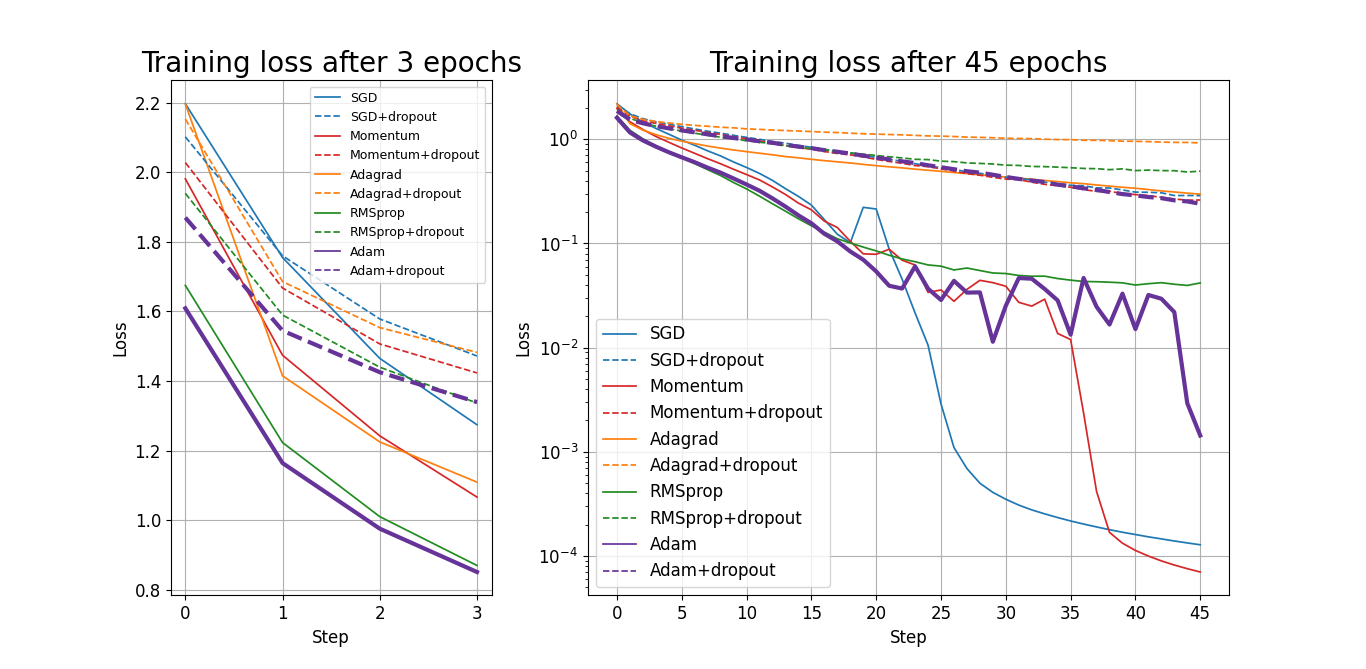
\includegraphics[width=140 mm]{images/cnn-nonwhitened.png}
	\caption{Kết quả thí nghiệm Convolutional Neural Network mà không thực hiện làm trắng ảnh.}
	\label{fig:exp-cnn-nonw}
\end{figure}

Kết quả của hình \ref{fig:exp-cnn-nonw} cho thấy độ lỗi Adam cao hơn khá nhiều khi bỏ qua bước làm trắng ảnh trong khi các thuật toán khác không bị ảnh hưởng nhiều. Như vậy, chúng ta có thể thấy việc làm trắng ảnh đầu vào sẽ giúp ích đáng kể cho quá trình huấn luyện khi sử dụng thuật toán Adam.

Về mặt thời gian tính toán, bảng \ref{tab:cnn-results} cho thấy với cùng một kích thước minibatch, có thể dễ hiểu khi SGD cho thời gian tính toán nhanh nhất vì thuật toán này chỉ tính gradient và cập nhật trọng số. Với Momentum, bước tính véc-tơ quán tính $v_t$ trước khi cập nhật trọng số làm tăng thời gian thực hiện mỗi epoch thêm khoảng 15$\%$. Bước tính đường chéo ma trận $G_t$ của các thuật toán tỉ lệ học thích ứng tốn nhiều thời gian hơn đáng kể, vì trong bước này còn có thao tác bình phương các phần tử trong véc-tơ gradient trước khi cộng dồn (thuật toán RMSprop có thêm bước nhân các phần tử này với hệ số suy biến). Adam kết hợp các bước tính quán tính trong Momentum và thích ứng tỉ lệ học, vì vậy Adam có thời gian thực thi chậm nhất trong tất cả các thuật toán.

Nhìn chung, chúng tôi có thể tái tạo các kết quả thí nghiệm mà bài báo công bố. Tuy nhiên, các kết quả tốt nhất của chúng tôi có độ lỗi thấp hơn đáng kể so với bài báo, đặc biệt là trong thí nghiệm Convolutional Neural Network. Vì chúng tôi không biết chính xác quá trình cài đặt và các siêu tham số đã được sử dụng trong bài báo gốc nên chúng tôi không thể khẳng định nguyên nhân của sự chênh lệch này. Chúng tôi cũng mở rộng thí nghiệm Convolutional Neural Network để tìm hiểu ảnh hưởng của việc làm tách biệt các đặc trưng của dữ liệu thông qua thao tác làm trắng ảnh lên quá trình huấn luyện.

\subsection{Phân tích độ lớn bước cập nhật của các trọng số trong rãnh hẹp}

Trong thí nghiệm này, chúng tôi kiểm chứng các khó khăn của dạng địa hình rãnh hẹp và cách mà các thuật toán khác nhau di chuyển trong đó. Vùng rãnh hẹp là vùng mà độ cong giữa các chiều có sự chênh lệch rất lớn. Cụ thể hơn, một số hướng sẽ có độ cong rất lớn trong khi các hướng khác lại rất bằng phẳng. Vì vậy, để có thể di chuyển hiệu quả trong địa hình này, chúng ta cần giảm kích thước bước cập nhật trên các chiều có độ cong lớn để tránh hiện tượng dao động, đồng thời cập nhật những bước dài hơn trên các chiều bằng phẳng có giá trị gradient nhỏ.

Chúng tôi sử dụng một hàm lỗi giả lập có 2 tham số với sự chênh lệch độ cong trên mỗi trục là rất lớn để tạo thành rãnh hẹp. Gradient mà các thuật toán sử dụng cũng sẽ là gradient của hàm mục tiêu tại vị trí đang xét. Vì vậy, đây có thể được coi như gradient của cả tập dữ liệu. Tất cả các thuật toán đều có cùng một điểm xuất phát.

\begin{figure}[htp]
	\centering
	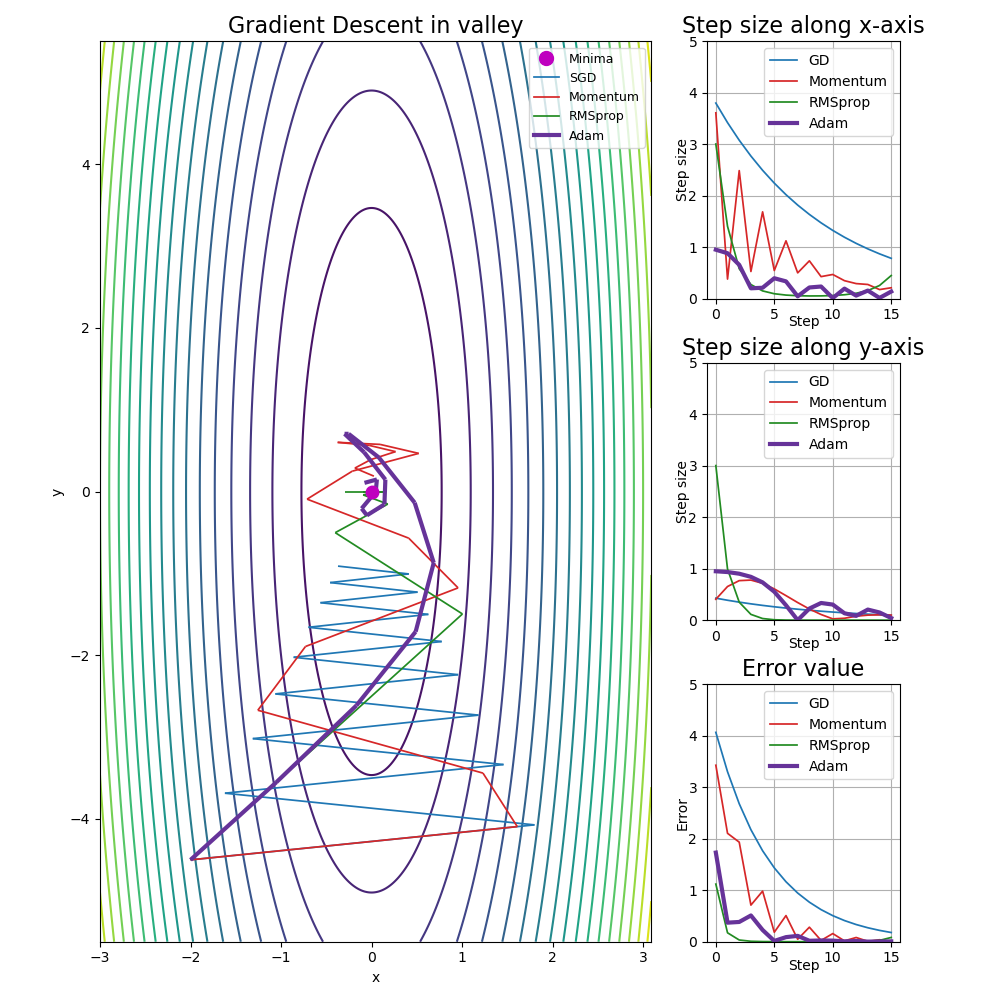
\includegraphics[width=140 mm]{images/step-size.png}
	\caption{Đường đi, độ lớn bước cập nhật theo từng chiều, và độ lỗi của các thuật toán trong quá trình tối ưu hàm giả lập.}
	\label{fig:aligned-step-size}
\end{figure}

Hình \ref{fig:aligned-step-size} cho thấy cách mỗi thuật toán di chuyển trong rãnh hẹp. GD rõ ràng là thuật toán gặp nhiều khó khăn nhất khi liên tục bị dao động giữa 2 bên vách. Độ lớn bước cập nhật trên trục $x$ của GD rất lớn, trong khi lượng cập nhật trên trục $y$ lại quá nhỏ khiến GD không đến được điểm cực tiểu. Momentum ban đầu cũng gặp khó khăn tương tự, nhưng nhờ quán tính kìm hãm lượng dao động trên trục $x$ đồng thời đẩy nhanh hơn trên $y$ nên Momentum di chuyển được tốt hơn. Với các thuật toán tỉ lệ học thích ứng, chúng ta có thể thấy RMSprop và Adam tối ưu độ lớn bước cập nhật trên cả trục $x$ và $y$ để di chuyển tốt hơn theo chiều dài của rãnh hẹp. Các biểu đồ độ lớn bước cập nhật cũng cho thấy rõ cách Adam kết hợp Momentum và RMSprop: vừa bước dài hơn theo trục $y$ và hạn chế di chuyển trên trục $x$, vừa kìm hãm dao động khi hướng của gradient thay đổi. Khi bị lố qua khỏi điểm cực tiểu, Adam cũng thực hiện đi ngược lại hiệu quả hơn Momentum.

\subsection{Phân tích đường đi trong rãnh hẹp có hướng trùng và không trùng với trọng số}

Từ nội dung đã trình bày ở Chương 3, các thuật toán tỉ lệ học thích ứng thay đổi tỉ lệ học theo từng trọng số riêng biệt. Vì vậy, dạng địa hình rãnh hẹp có các hướng trùng với trục của trọng số sẽ là trường hợp mà các thuật toán tỉ lệ học thích ứng phát huy hiệu quả cao nhất. Ngược lại, trường hợp rãnh hẹp chéo góc so với các trục của trọng số sẽ gây ra nhiều khó khăn nhất cho các thuật toán ấy.

Trong thí nghiệm này, thay vì tối ưu trực tiếp trên hàm giả lập, chúng tôi tạo một bộ dữ liệu ngẫu nhiên gồm 10000 phần tử có phân phối đều trên một trục, với giá trị của các điểm dữ liệu trên trục còn lại được quyết định bởi một hàm có 2 tham số. Mức độ chênh lệch giữa 2 tham số sẽ tạo ra địa hình rãnh hẹp, và sự phụ thuộc giữa các tham số trong hàm sẽ khiến cho các chiều của rãnh hẹp không còn trùng với tham số. Chúng tôi thực hiện ``fit'' một đường thẳng hồi quy trên bộ dữ liệu này bằng phương pháp Stochastic Gradient Descent. Kích thước minibatch mà chúng tôi sử dụng là 50.

\begin{figure}[htp]
	\centering
	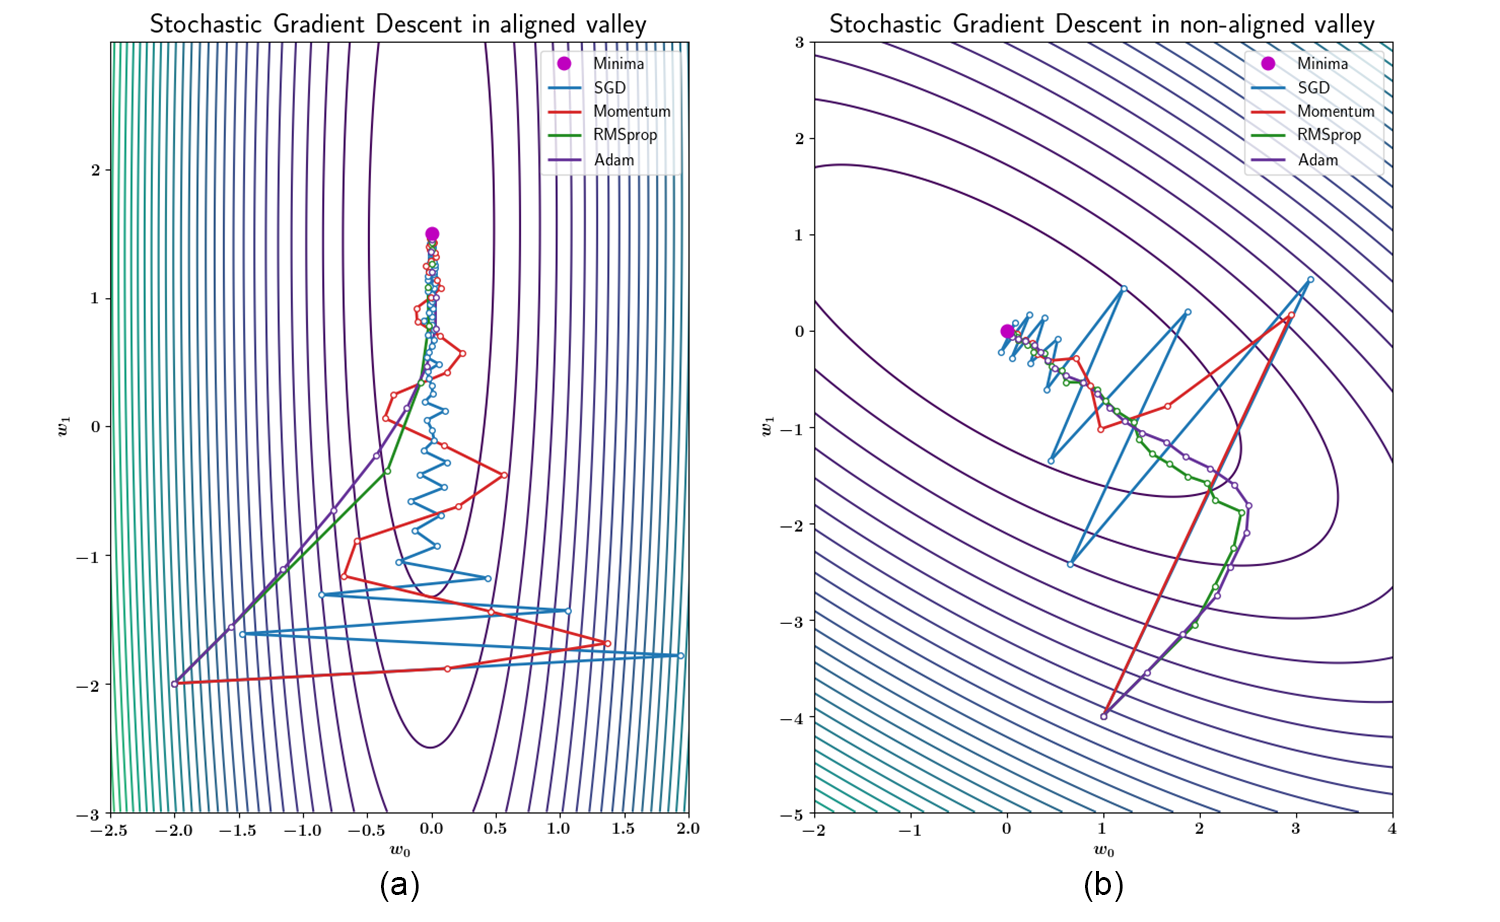
\includegraphics[width=140 mm]{images/aligned-nonaligned.png}
	\caption{Đường đi của các thuật toán trong rãnh hẹp có hướng trùng với trọng số (a) và không trùng với trọng số (b).}
	\label{fig:aligned-nonaligned}
\end{figure}

Hình \ref{fig:aligned-nonaligned}a cho thấy kết quả tương tự thí nghiệm trước, với Adam và RMSprop bước những bước dài hơn trên hướng bằng phẳng của rãnh hẹp (tương ứng với trục $w_1$) trong khi SGD và Momentum bị dao động và rất khó di chuyển theo trục $w_1$. Tuy nhiên, vì sử dụng gradient của các minibatch để di chuyển nên sự dao động của SGD và Momentum cũng có phần được cải thiện hơn so với thí nghiệm trước sử dụng gradient của bề mặt lỗi.

Trong trường hợp các hướng của rãnh hẹp không trùng với trục của trọng số (hình \ref{fig:aligned-nonaligned}b), chúng ta có thể thấy Adam và RMSprop gặp nhiều khó khăn hơn trong việc điều chỉnh tỉ lệ học. Adam và RMSprop chỉ thực hiện những bước cập nhật rất nhỏ. Cũng vì những bước cập nhật quá nhỏ mà Adam cũng không thể tích tụ được lượng quán tính để tăng tốc, vì vậy các bước đi của Adam và RMSprop khá tương đồng với nhau. SGD và Momentum hầu như không bị ảnh hưởng bởi hướng của rãnh hẹp.

\subsection{Vấn đề đặc trưng thưa và nhiễu}

Đặc trưng thưa là những đặc trưng mang giá trị 0 hoặc gần bằng 0 tại đa số các điểm dữ liệu; ngược lại, ta có đặc trưng đặc. số lần các đặc trưng thưa được cập nhật là rất ít hoặc cập nhật với lượng rất nhỏ, từ đó kéo dài quá trình huấn luyện mạng nơ-ron nhiều tầng ẩn. Thêm nữa, đặc trưng thưa xuất hiện ở hầu hết các mạng nơ-ron sâu hiện nay. Đó là lý do tại sao vấn đề về đặc trưng thưa này cần được giải quyết.

\begin{figure}[htp]
	\centering
	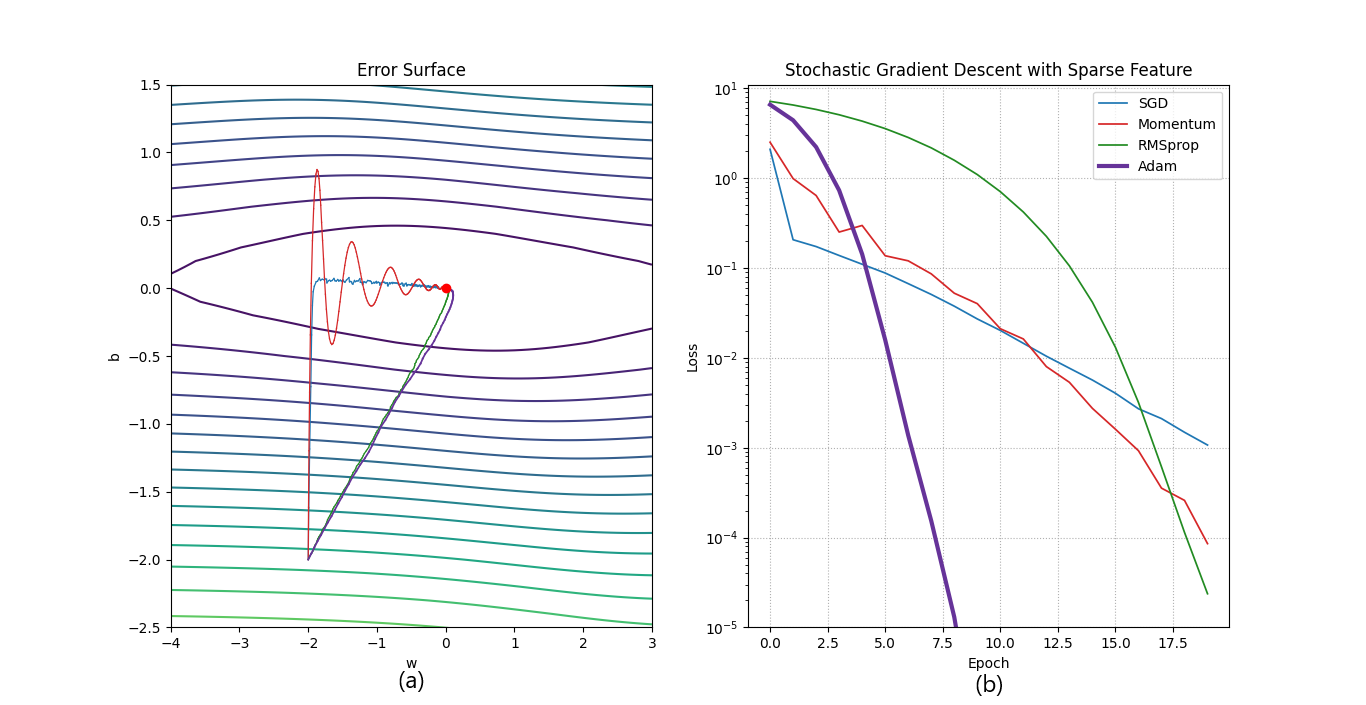
\includegraphics[width=140 mm]{images/sparse.png}
	\caption{Đường đi của các thuật toán trong bề mặt lỗi (trái) và độ lỗi (phải) của từng thuật toán trong trường hợp đặc trưng thưa.}
	\label{fig:sparse}
\end{figure}

Để quan sát cách các thuật toán tối ưu hoạt động với dữ liệu thưa, thí nghiệm sử dụng dữ liệu là $n$ cặp $(x,y)$ được khởi tạo ngẫu nhiên. Sau đó, chọn 80$\%$ trong số $n$ cặp và gán giá trị $x = 0$ với mục đích là khiến cho đặc trưng $x$ thưa. Sử dụng mô hình hồi quy tuyến tính với hàm mục tiêu có dạng $y = wx + b$, các thuật toán được sử dụng để tối ưu hàm chi phí $MSE = \frac{1}{n}\sum_{i=1}^n(y - wx - b)^2$. Kết quả sau 60 epoch được thể hiện như trong hình \ref{fig:sparse}b và hình \ref{fig:sparse}a thể hiện đường đi của các thuật toán trên bề mặt lỗi.

Các thuật toán tối ưu như SGD không hoạt động tốt đối với dữ liệu mà số lượng dữ liệu thưa lớn. Vì các thuật toán này sử dụng thông tin của gradient để thực hiện bước cập nhật, và chính thông tin này bị mất đi hoặc có rất ít trong dữ liệu thưa. Sự thiếu hụt thông tin làm cho các thuật toán SGD hay Momentum thực hiện những bước đi rất nhỏ tại hướng tương ứng với đặc trưng này. Đó là lý do vì sao trong hình \ref{fig:sparse}a cho ta thấy thuật toán Momentum cập nhật nhanh tại hướng tương ứng với đặc trưng đặc $b$ nhưng lại đi những bước rất nhỏ theo hướng của đặc trưng thưa $w$. Vì thực hiện những bước cập nhật lớn trên hướng $b$ nên độ lỗi của Momentum giảm rất nhanh trong các bước đầu tiên. Tuy nhiên, độ lỗi giảm chậm tại những bước tiếp theo ứng với các bước di chuyển chậm chạp theo hướng $w$.

Bằng việc sử dụng tỉ lệ học riêng biệt cho từng hướng, thuật toán RMSprop và Adam tăng nhanh tốc độ cập nhật tại hướng $w$ từ đó tăng tốc quá trình huấn luyện. Vì RMSprop và Adam đảm bảo cả hai hướng $w$ và $b$ đều được cập nhật nên đường đi của hai thuật toán trên bề mặt lỗi \ref{fig:sparse}a là một đường chéo hướng thẳng về cực tiểu. Tuy nhiên Adam nhờ có thêm yếu tố momentum mà cho đường đi thẳng hơn về phía cực tiểu. Độ lỗi của thuật toán RMSprop mặc dù giảm nhanh hơn Momentum nhưng thuật toán hội tụ tại điểm có độ lỗi cao hơn. Giải thích cho hiện tượng này là do RMSprop gặp dao động tại vùng gần cực tiểu và không thể hội tụ về điểm cực tiểu. Bên cạnh đó, mặc dù Adam có tốc độ chậm hơn Momentum nhưng lại có thể hội tụ về điểm cực tiểu nhanh hơn. Một lý do là vì Adam sử dụng EMA nên cần một thời gian để có thể xấp xỉ tốt hơn. Tuy nhiên, đó không phải là nguyên nhân chính. Một lý do khác là vì bước cập nhật của Adam trên hướng có độ dốc cao b chậm hơn so với Momentum nhưng lại có những bước đi có ý nghĩa hơn Momentum theo hướng tối ưu có độ dốc thấp $w$. Kết quả là Adam có thể hội tụ tại cực tiểu tốt hơn và nhanh hơn Momentum.

\begin{figure}[htp]
	\centering
	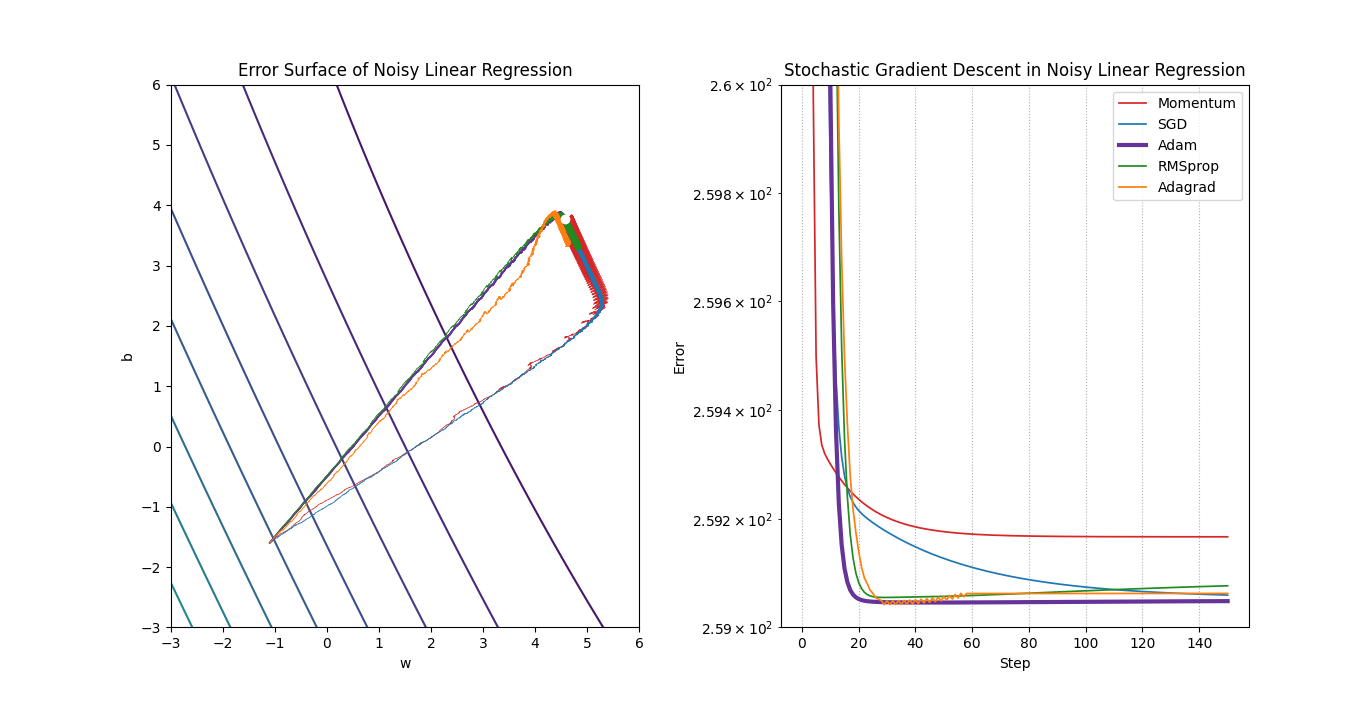
\includegraphics[width=140 mm]{images/noise.png}
	\caption{Đường đi của các thuật toán trong bề mặt lỗi (a) và độ lỗi của từng thuật toán trường hợp nhiều nhiễu (b).}
	\label{fig:noise}
\end{figure}

Một khó khăn khác khi huấn luyện mạng nơ-ron là huấn luyện trên dữ liệu nhiều nhiễu. Để thực hiện quan sát cách các thuật toán xử lý nhiễu, thí nghiệm sử dụng một tập dữ liệu gồm $n$ cặp $(x,y)$ với $y$ là giá trị nhãn. Sau đó, thực hiện thêm nhiễu vào trong giá trị $y$ để cho ra $\hat y$ là giá trị mà ta quan sát được. Mô hình sử dụng linear regression và hàm chi phí MSE để huấn luyện dựa trên $n$ cặp $(x,\hat y)$. Kết quả được mô tả trong hình \ref{fig:noise} sau 150 epochs. Ta dễ dàng nhận thấy được Momentum thực hiện bước cập nhất đầu rất nhanh nhưng sau đó lại hội tụ tại một điểm có độ lỗi cao hơn Adam và RMSprop. Ta nhận thấy trong \ref{fig:noise}b, Adam và RMSprop cùng hội tụ về cùng độ lỗi nhưng do Adam có thêm quán tính mà thời gian hội tụ sớm hơn. Vẫn chưa có lý do tại sao các thuật toán tỉ lệ học thích ứng lại có thể hoạt động tốt trong trường hợp này. Một bài báo của Balles Lukas và Hennig Phillip \cite{balles2018dissecting} cho rằng vì Adam không thực sự sử dụng kết quả của gradient mà thay vào đó xác định hướng chỉ dựa vào dấu của gradient. Chính vì vậy mà Adam không bị ảnh hưởng bởi độ nhiễu có trong dữ liệu trong khi Momentum cố gắng fit nhiễu vào trong kết quả dự đoán. Đây được coi là lý do tại sao Momentum hội tụ tại một điểm có độ lỗi cao hơn.

\subsection{Huấn luyện mô hình VGG16}

Chúng tôi thực hiện huấn luyện kiến trúc mạng tích chập nhiều tầng ẩn VGG16 của Karen Simonyan và Andrew Zisserman \cite{simonyan2014verydeep} trên tập dữ liệu ImageNet. Đây là một kiến trúc mạng nơ-ron nhiều tầng ẩn được sử dụng rộng rãi trong rất nhiều bài toán khác nhau, không chỉ riêng bài toán phân lớp do khả năng trích xuất đặc trưng rất mạnh. Kiến trúc mạng VGG16 cũng thường được sử dụng làm thước đo đánh giá độ hiệu quả của các thuật toán huấn luyện mạng nơ-ron nhiều tầng ẩn \cite{zhuang2020adabelief} \cite{schneider2018deepobs}. Các thiết lập huấn luyện như kích thước minibatch, kích thước và quá trình tiền xử lý ảnh đầu vào được giữ nguyên như trong bài báo gốc của VGG16 \cite{simonyan2014verydeep}.

Với mỗi thuật toán tối ưu, chúng tôi cố gắng dò tìm bộ siêu tham số cho kết quả tốt nhất. Tuy nhiên, do việc huấn luyện mạng VGG16 với khoảng 138 triệu tham số trên một tập dữ liệu lớn như ImageNet rất tốn kém nên chúng tôi không thể dò tìm siêu tham số một cách chi tiết như các thí nghiệm khác. Một trường hợp đặc biệt là thuật toán SGD dường như không thể tối ưu cho kiến trúc mạng này khi độ lỗi luôn giữ ở mức cao bất kể siêu tham số mà chúng tôi thử nghiệm, vì vậy chúng tôi không bao gồm biểu đồ của SGD trong kết quả. Các siêu tham số được sử dụng trong thí nghiệm được trình bày trong bảng \ref{tab:vgg16-hparam}

\begin{figure}[htp]
	\centering
	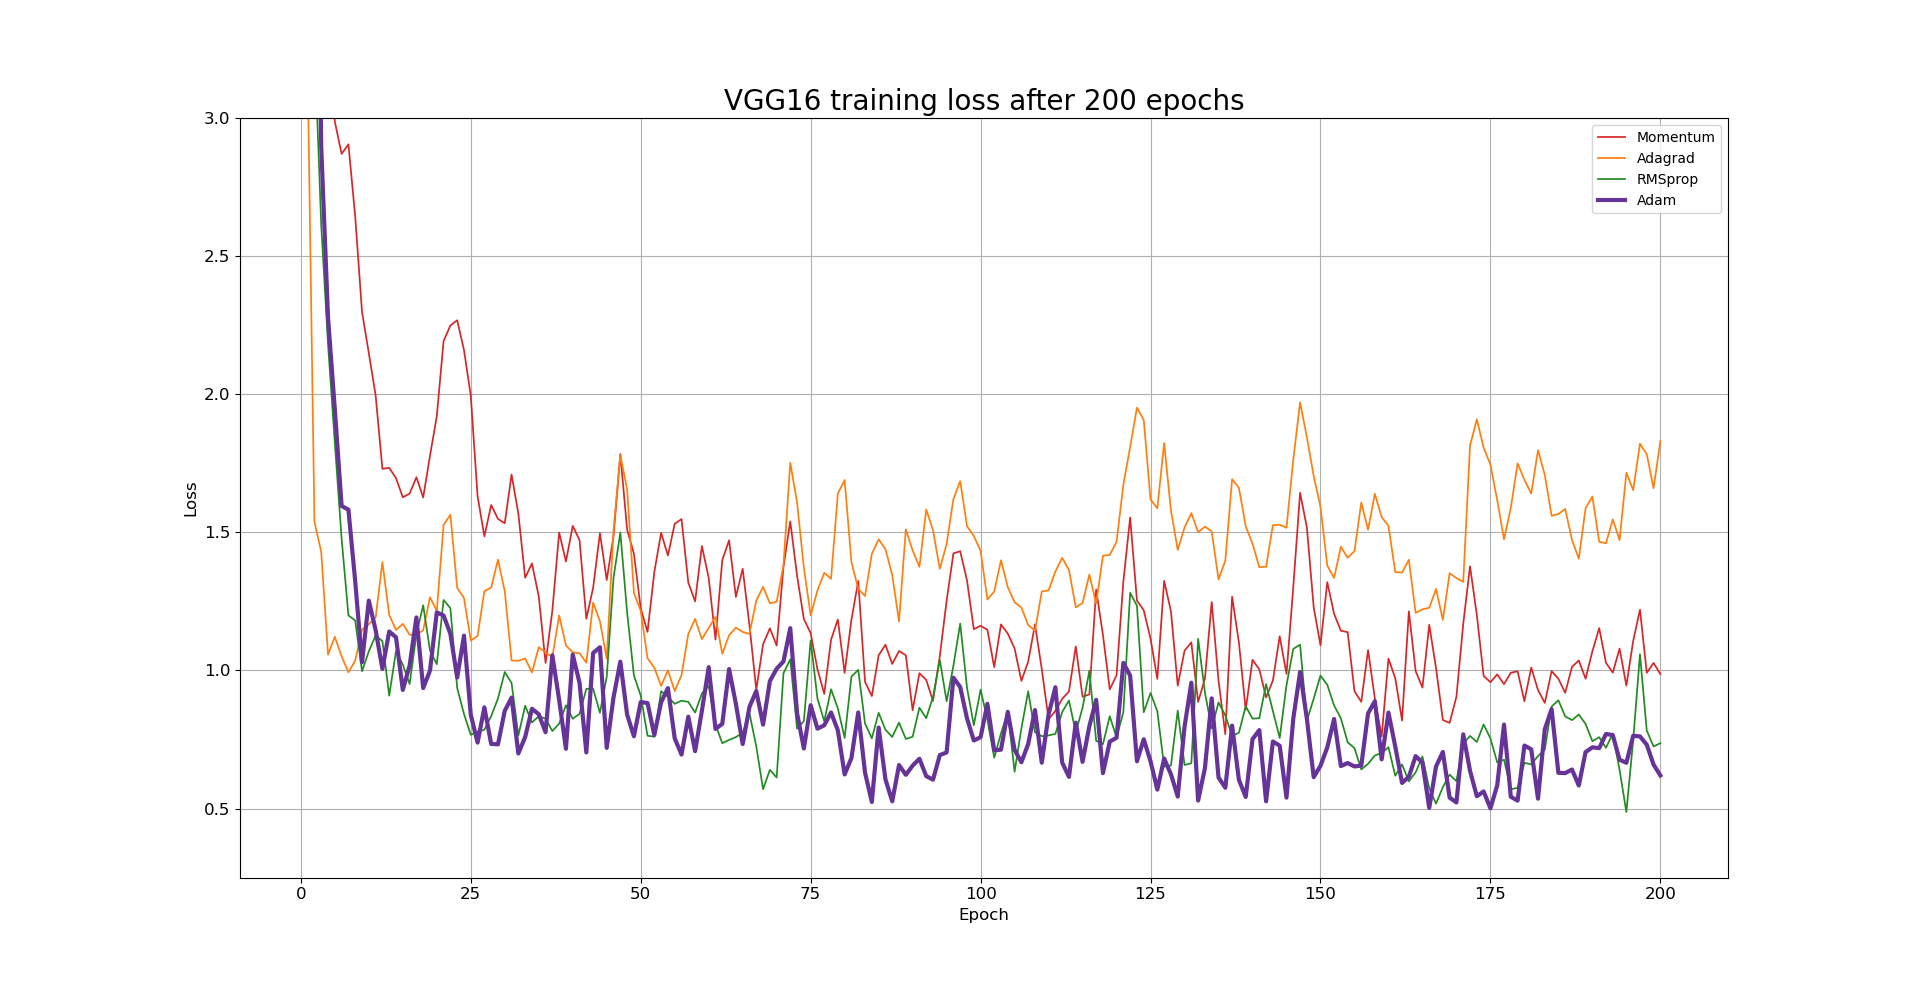
\includegraphics[width=140 mm]{images/vgg16.png}
	\caption{Đường đi của các thuật toán trong bề mặt lỗi (trái) và độ lỗi (phải) của từng thuật toán trong trường hợp đặc trưng thưa.}
	\label{fig:vgg16-loss}
\end{figure}

Quá trình huấn luyện mô hình VGG16 trên tập dữ liệu ImageNet (hình \ref{fig:vgg16-loss}) cho thấy Adam là thuật toán tối ưu hiệu quả nhất trong số các thuật toán được thí nghiệm khi có độ lỗi giảm nhanh chóng và ổn định. Adagrad và Momentum bị dao động mạnh trong suốt quá trình huấn luyện và không đạt được độ lỗi thấp. Chỉ có RMSprop là có độ lỗi gần với Adam nhất, nhưng RMSprop cũng có biên độ dao động lớn hơn.

\subsection{Huấn luyện mô hình ngôn ngữ}

Chúng tôi sử dụng thiết lập giống trong bài báo của Zaremba và cộng sự \cite{zaremba2014recurrent} cho mô hình LSTM-medium. Sử dụng kiến trúc mạng RNN gồm 2 tầng Long Short-term Memory (LSTM), mỗi tầng có 650 nơ-ron với số bước unroll là 35. Chúng tôi khởi khởi tạo hai tầng ẩn này bằng giá trị 0 và sử dụng trạng thái ẩn cuối cùng của minibatch $t$ làm giá trị khởi tạo của trạng thái ẩn của minibatch $t+1$ với kích thước của một minibatch là 20.

Các giá trị trọng số trong mạng được khởi tạo theo phân phối đều trong khoảng [-0.05,0.05]. Với tỷ lệ dropout là 0.5 cho các liên kết không hồi quy, mô hình được huấn luyện trong 39 epoch với tỷ lệ học được tuning tốt nhất cho mỗi thuật toán tối ưu và được trình bày trong bảng \ref{tab:ptb-hparam}. Trong quá trình huấn luyện, sau epoch thứ 6 thì tỷ lệ học sẽ được nhân với $\frac{5}{6}$ sau mỗi epoch. Giá trị clip của gradient được sử dụng là 5.

\begin{figure}[htp]
	\centering
	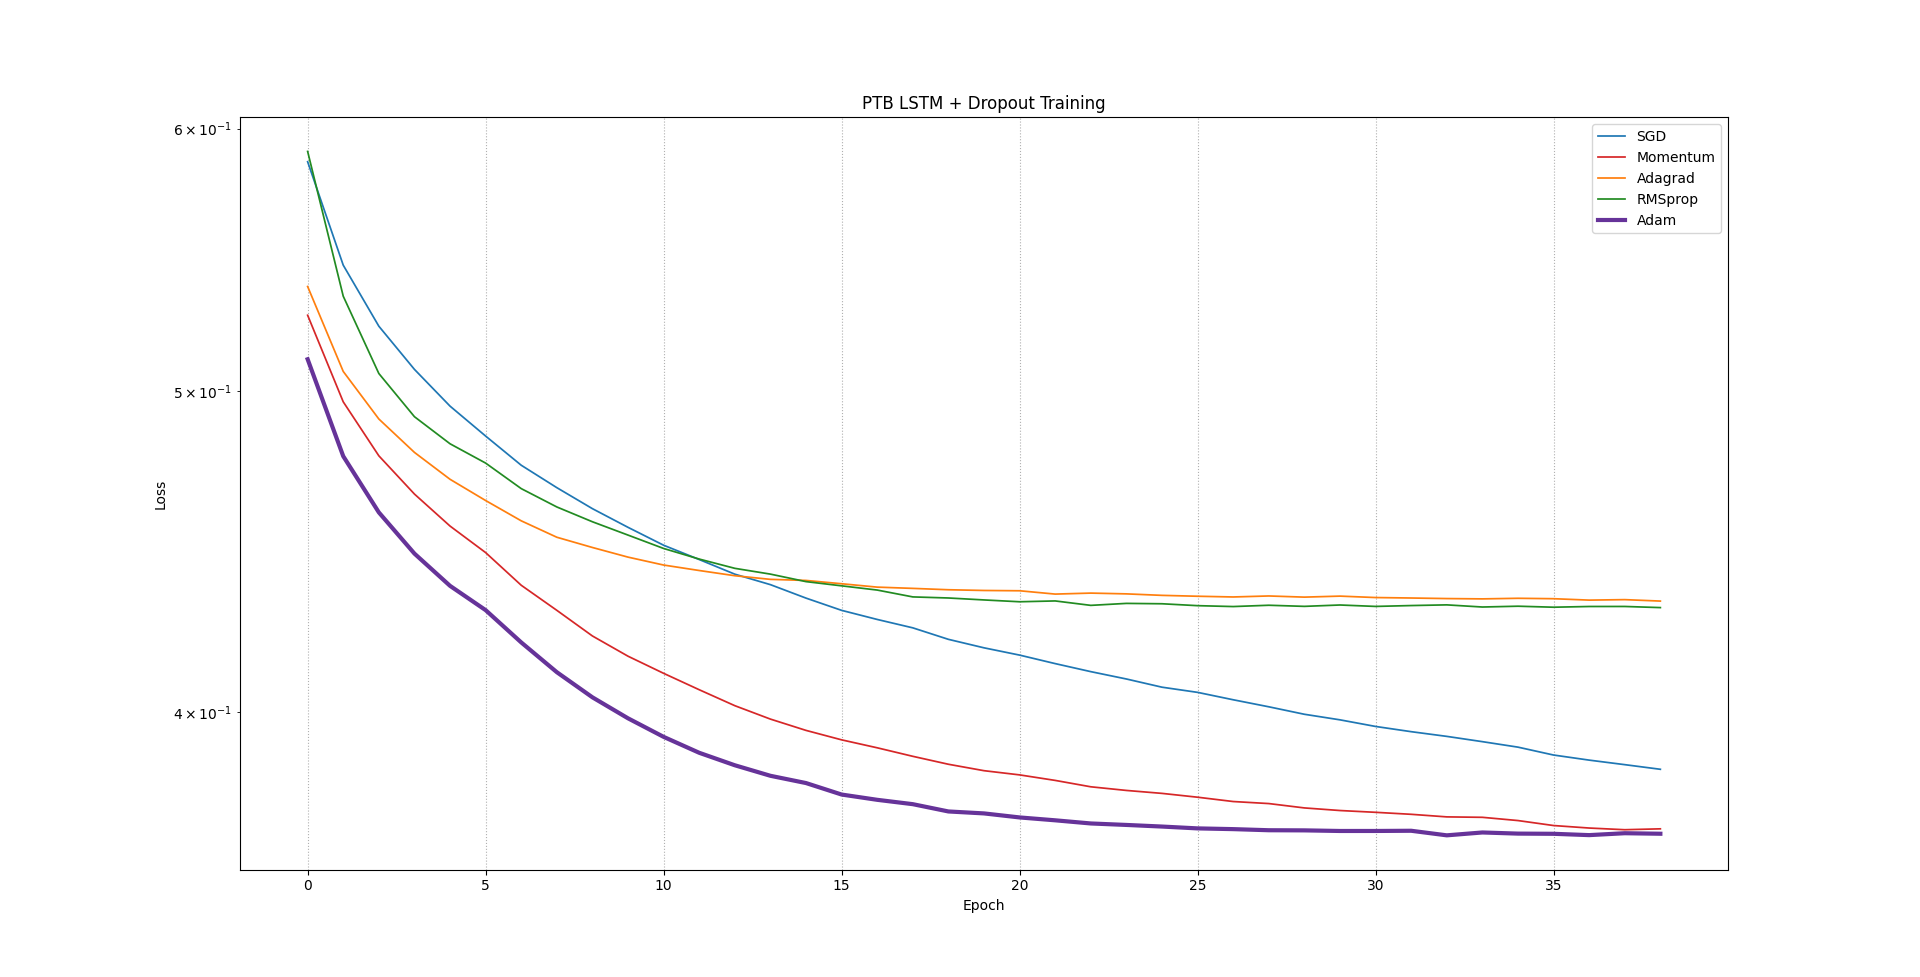
\includegraphics[width=140 mm]{images/ptb.png}
	\caption{Mô tả kết quả thí nghiệm của mô hình ngôn ngữ trên tập dữ liệu Penn Treebank gồm kết quả trên tập huấn luyện (trái) và tập kiểm thử (phải).}
	\label{fig:ptb}
\end{figure}

Hình \ref{fig:ptb} cho ta kết quả chạy của mô hình LSTM trên tập Penn Tree Bank trong 39 epoch. Từ đó, ta thấy được rằng Adam cho độ lỗi nhỏ nhất ngay từ những epoch đầu tiên, theo ngay sau đó là Momentum. Mặc dù RMSProp cho độ lỗi giảm mạnh nhưng rất nhanh chững lại và không thể xuống điểm có độ lỗi thấp hơn nữa.